
\arrayrulecolor{black!20}
\renewcommand{\labelitemi}{\textbullet} % Utilise le symbole point
% \renewcommand{\tabularxcolumn}[1]{>{\arraybackslash\vspace{4pt}}m{#1}
% \renewcommand{\thesection}{\arabic{chapter}.\arabic{section}}<{\vspace{4pt}}}
\chapter{CADRE GÉNÉRAL DU PROJET}
\indent Ce chapitre introductif a pour but de situer le projet dans son environnement organisationnel et contextuel. Il présente dans sa première partie l'organisme d'accueil, les différentes formations que nous avons suivies pour être aptes à intégrer les équipes, de mettre en évidence le contexte général du projet, sa problématique ainsi que ses objectifs. Il éclaire également sur l'équipe de travail, la méthodologie adoptée pour la gestion du projet tout au long de la durée du stage, et les outils utilisés pour le suivi. Ces éléments ont pour but de fournir les bases nécessaires pour une compréhension approfondie et une mise en contexte de mon projet de PFE réalisé au sein de SQLI.

\newpage
\label{chap:premierchapitre}

\section{Présentation de l’entreprise d’accueil SQLI}
\indent Cette section initiale met en lumière le Groupe SQLI en mettant l'accent sur ses activités clés, son chiffre d'affaires ainsi que ses clients. Ensuite, nous nous concentrerons spécifiquement sur SQLI Maroc et ses valeurs clés.
\subsection{Groupe SQLI}

\indent SQLI est une entreprise européenne de services numériques fondée en 1990 par Jean Rouveyrol et Alain Lefebvre. Elle se spécialise dans la conception, le développement et le déploiement de solutions digitales visant à créer des expériences unifiées \cite{1}. Avec un effectif de 2400 collaborateurs répartis dans 13 pays, SQLI bénéficie d'une présence internationale solide.\par

\begin{figure}[H]  
  \centering  
  \includegraphics[height=1.5cm,width=0.1\linewidth]{sqliligo-removebg-preview.png}
  \caption{Logo de SQLI}
  \label{Logo SQLI}
\end{figure}
% \vspace{0.3cm}
\indent SQLI est un groupe européen de services numériques spécialisé dans la conception, le développement et le déploiement de dispositifs digitaux créateurs d’expériences unifiées. Créé par Jean Rouveyrol et Alain Lefebvre, le groupe compte 2100 collaborateurs répartis dans 13 pays. Avec une présence internationale robuste, SQLI occupe une position de premier plan dans le monde du numérique.
SQLI se distingue par trois valeurs fondamentales : l'Esprit créatif, l'Engagement et la Pensée prospective. Ces principes jouent un rôle essentiel dans le succès de l'entreprise, propulsant son innovation au-delà des conventions et façonnant des expériences digitales uniques et inspirantes.


\subsubsection{Activités du groupe}

\indent SQLI Digital Experience propose une gamme complète de services pour accompagner ses clients dans leur transformation digitale. Initialement spécialisée dans les solutions e-commerce, l'entreprise s'est progressivement diversifiée pour offrir des services de conseil en stratégie digitale, de développement d’applications, de gestion de contenu, de marketing digital et de transformation numérique.


\subsubsection{Chiffre Clés du groupe}

\indent Les chiffres clés suivants présentent la situation actuelle de SQLI :

\begin{itemize}
    \item Avec 33 ans d’expérience et d’innovation, SQLI place son développement sur une expertise technologique de pointe et sur une politique intense de veille.
    \item SQLI compte plus de 2400 collaborateurs répartis dans 13 pays, dont la France, l'Angleterre, la Suède, les Pays-Bas, l'Espagne, l'Allemagne, la Belgique, le Luxembourg, la Suisse et le Maroc.
    \item En 2022, le groupe SQLI a enregistré un chiffre d’affaires de 251,2 millions de dollars. Cette performance a été rendue possible grâce à une offre parfaitement adaptée aux attentes du marché et à une reprise progressive de la demande de services informatiques.
    \vspace{0.5cm}
\end{itemize}
\begin{figure}[H]  
  \centering  
  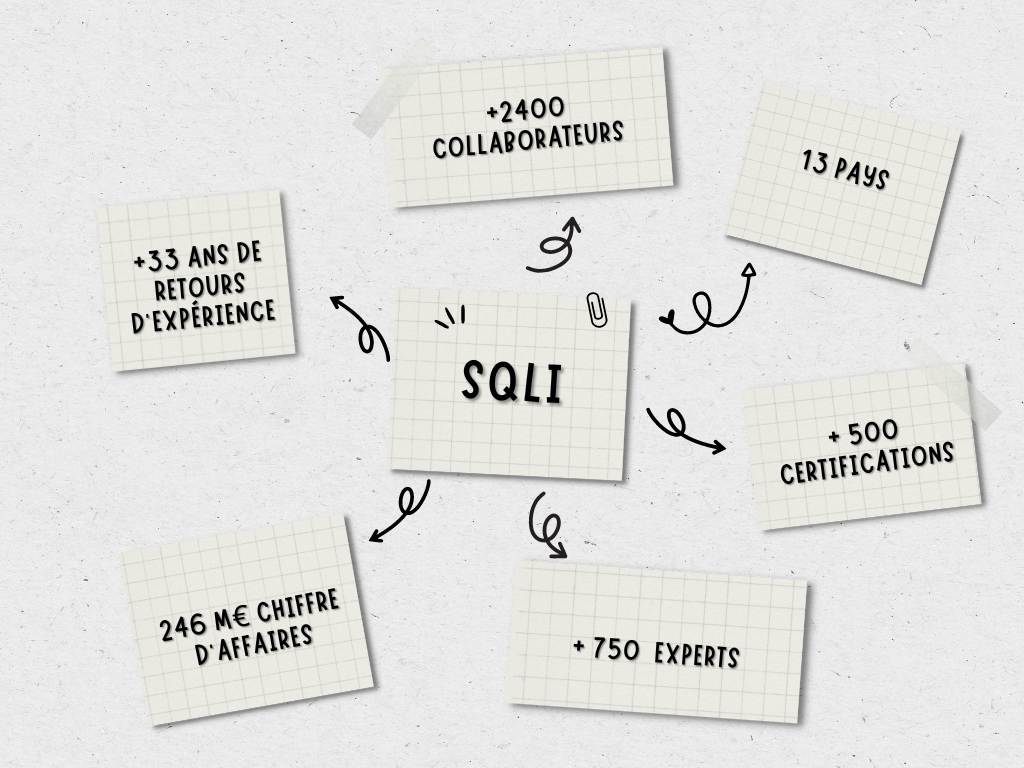
\includegraphics[height=6cm,width=0.4\linewidth]{images/chap1/cle chiffre.png}
  \caption{Chiffre Clés de SQLI}
  \label{Logo SQLI}
\end{figure}

\subsubsection{Clients du groupe}

\indent  Les valeurs de SQLI reposent sur des qualités humaines solides telles que le respect de l’autre, l’esprit d’équipe, l’authenticité des échanges, la détermination ainsi que le plaisir au quotidien :
\begin{itemize}
  \item Engagement : Chez SQLI, l’engagement s’étend également à l’égard de ses clients. Il est lié à l’esprit de service et à la volonté constante d’imaginer et de leur apporter les meilleures solutions.
  \item Pensée prospective : Il s'agit de la capacité à anticiper, à penser en avance et plus loin. Au sein de SQLI, la pensée prospective puise ses fondements dans l'expertise et l'expérience des collaborateurs.
  \item Esprit créatif : Intimement lié à l’ouverture aux autres et à ce qui est singulier, l’esprit créatif chez SQLI est également nourri par l’esprit d’équipe.
  \vspace{0.5cm}
\end{itemize}
\begin{figure}[H]  
  \centering  
  
\includegraphics[height=5cm,width=0.4\linewidth]{images/chap1/sqli partenaire .png}
  \caption{Clients de groupe \cite{1}}
  \label{Logo SQLI}
\end{figure}

\subsubsection{Clients du groupe}

\indent  Dans le cadre du développement continu de son activité, SQLI accorde une importance primordiale à la diversité de sa clientèle et des secteurs d’activité qu’elle couvre, afin de limiter le risque de dépendance à un nombre restreint de clients. Ainsi, SQLI compte plus de 1200 clients issus de tous les secteurs d’activité, notamment les services, l’industrie, les banques et assurances, les administrations et services publics, la distribution et les transports. Cette variété de clients témoigne de la confiance accordée à SQLI par une multitude d'acteurs économiques. En effet, SQLI réunit toutes les compétences nécessaires pour mener à bien les projets de ses clients, de la consultation à la réalisation, en passant par la conception, l'interface utilisateur, la formation et l'ergonomie.
\begin{figure}[H]  
  \centering  
  
\includegraphics[height=5cm,width=0.4\linewidth]{images/chap1/sqli partenaire .png}
  \caption{Clients de groupe \cite{1}}
  \label{Logo SQLI}
\end{figure}



\subsubsection{Partenaires du groupe}


\indent Le positionnement du groupe SQLI à l'intersection du monde du digital et du système d’information de l’entreprise constitue sa valeur ajoutée. Le groupe a tissé un réseau de partenaires afin de relever ses défis de la manière la plus performante possible, et ainsi offrir le meilleur conseil et les meilleures solutions.
\begin{figure}[H]  
  \centering  
  
\includegraphics[height=5cm,width=0.4\linewidth]{images/chap1/sqli partenaire .png}
  \caption{Clients de groupe \cite{1}}
  \label{Logo SQLI}
\end{figure}


\subsection{SQLI Maroc}
\indent  SQLI Maroc, créée en 2003 à Rabat par Eric Chanal, représente le centre de Delivery et d'Innovation du Groupe SQLI. Bénéficiant d'une solide expertise et d'une grande expérience, l'entreprise est présente sur trois sites stratégiques : Rabat, où nous avons eu l'opportunité d'effectuer notre stage PFE, Oujda et Casablanca.   Voici sa fiche technique:



% l'ajoute de titre de tableau avec space between titre de tab et le tab
\captionsetup{type=table}
\captionof{table}{Fiche technique de SQLI Maroc}
\vspace{0.3cm}
% tab
\begin{center}
\begin{tabularx}{17cm}{|X|X|}

  \hline
  
 \textbf{Dénomination sociale}  & \textbf{SQLI Digital Experience} \\
  \hline{Année de fondation} & 2003  \\
  \hline
  {Fondateur}& Eric Chanal  \\

  \hline
{Siège social} & Rabat, Maroc\\
 \hline  
 {Activité} & Conseil en systèmes et logiciels informatiques.\\
  
  \hline  
{Effectif des employés} & Plus de 900 collaborateurs.\\
  \hline
 {Sites d'implantation} & Rabat, Oujda et Casablanca.\\
 
  \hline
 {Site web} & https://www.sqli.com/fr-fr\\
  \hline
   {Téléphone} & Pour le bureau de Rabat : +212 537
619 710 \\
  \hline
  \end{tabularx}
  \end{center}

  % \subsubsection{Départements de SQLI}

\vspace{0.5cm}
\indent SQLI Maroc comprend principalement deux structures essentielles, à savoir :

\begin{enumerate}
    \item \textbf{SQLI WAX INTERRACTIVE} : S’occupe à accompagner les clients sur la voie de digitalisation afin d’avoir un bon positionnement sur le marché. Cette structure
     intervient sur le plan stratégique vis-à-vis les clients.
     \item \textbf{SQLI ENTREPRISE} : Cette entité est chargée de la mise en œuvre des systèmes d'information pour les clients. Elle se compose de plusieurs Business Units spécialisées dans différents domaines :
\begin{itemize}

    \item \textbf{E-commerce/ JAVA EE} : se focalise sur la création et la mise en place de sites de e-commerce ainsi que sur le développement d'applications utilisant la technologie JAVA EE.
    \item \textbf{Mobile/Front} : spécialise dans le développement d'applications mobiles et de l'interface utilisateur (Front-end) pour les clients.
     \item \textbf{Microsoft} : se charge de la réalisation d'applications basées sur les technologies Microsoft.
      \item \textbf{Agency} : joue un rôle transversal en assurant la conception de l'interface utilisateur (Front-end) pour toutes les autres Business Units.
        \item \textbf{Delivery} : se charge de la gestion des livraisons et des recettes vis-à-vis des clients.       
\end{itemize}
\end{enumerate}
\vspace{0.5cm}
\begin{figure}[H]  
  \centering  
  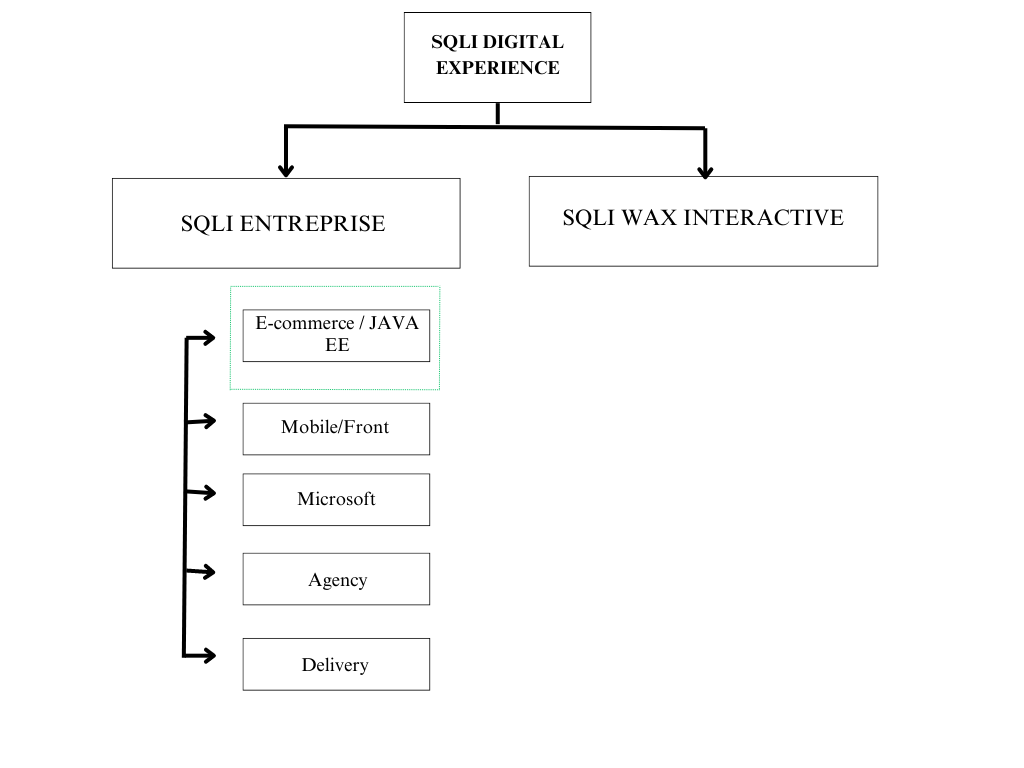
\includegraphics[height=6cm,width=0.6\linewidth]{images/chap1/departement.png}
  \caption{Départements de SQLI}
  \label{Over The Air updates}
\end{figure}

\indent  Notre stage de fin d'études s'est déroulé dans le département Java JEE, qui regroupe plusieurs projets destinés à de grandes entreprises clientes.
\section{Présentation du projet}

\subsection{Étude de l'existant}
\indent La plateforme Chanel offre une diversité de choix de paiement aux clients suisses, notamment les cartes de crédit renommées telles que \textbf{Mastercard}, \textbf{Visa} et \textbf{American Express}, ainsi que les options \textbf{PayPal} et \textbf{Apple Pay}. 

\indent  &\  &\  &\ Notre projet vise à intégrer la méthode de paiement \textbf{TWINT}, largement adoptée en Suisse, dans le site de e-commerce de la célèbre marque Chanel, une entreprise de renommée mondiale opérant dans divers secteurs tels que la haute couture, les parfums, les produits de luxe, les accessoires et le prêt-à-porter.

\begin{figure}[H]  
  \centering  
  \includegraphics[height=2cm,width=0.3\linewidth]{EXistant.png}
  \caption{Modes de paiement}
  \label{Over The Air updates}
\end{figure}

\subsection{Objectif et problématique du projet}
 \indent  &\  &\  &\ Le but de ce projet consiste à intégrer la méthode de paiement TWINT dans le site du client, qui repose sur la plateforme SAP Hybris, en utilisant l'API fournie par le prestataire de services de paiement \textbf{Adyen}.

\indent  &\  &\  &\  L'intégration de Twint dans le site e-commerce est motivée par plusieurs facteurs essentiels. premièrement, Twint est devenu une option de paiement extrêmement populaire en Suisse. Deuxièmement, Twint offre une expérience de paiement simple, rapide et sécurisée. Enfin, en intégrant ce mode de paiement, nous élargissons notre gamme d'options de paiement pour mieux répondre aux besoins de nos clients.

\indent  &\  &\  &\ Ainsi,la problématique qui se pose est \textbf{Comment intégrer efficacement TWINT au sein du site e-commerce Chanel, spécifiquement pour le marché suisse, tout en maintenant la cohérence avec la structure de code existante et en respectant les conventions et normes de développement établies, afin de garantir une intégration harmonieuse sans compromettre la stabilité et les performances du système existant ?}


\begin{comment}

\section{Conduite du projet}
\subsection{Equipe Cart, Checkout \& Payment}

\indent Après ma période de formation, j'ai intégré l'équipe "Cart, Checkout and Payment" du projet "Chanel One" en tant que développeur backend. Cette équipe fait partie d'un projet plus vaste comprenant 15 équipes de fonctionnalités différentes.\par
\indent Notre équipe se concentre spécifiquement sur le processus de commande et de paiement, tandis que les autres équipes se consacrent à d'autres aspects du projet. Ainsi, la collaboration entre les différentes équipes a permis de créer une solution complète et cohérente. Egalement, au sein de notre équipe, nous travaillons en étroite collaboration avec un Scrum Master, un expert technique, un product owner, un développeur frontend et deux assurances qualité, ce qui favorise le développement d'une solution robuste et performante.\par
\indent La structure de l'équipe est illustrée dans le schéma ci-dessous:
\begin{figure}[H]  
  \centering 
  \includegraphics[height=8cm,width=0.6\linewidth]{images/chap1/structure.png}
  \caption{Structure de l’équipe Cart, Checkout and Payment }
  \label{Over The Air updates}
\end{figure}
\subsection{Méthodologie de travail : Scrum}

\indent  Dans le processus de sélection de notre 
méthodologie de gestion de projet, Nous avons choisi la méthode Scrum pour sa flexibilité et son adaptation aux besoins métiers changeants. Contrairement aux méthodologies traditionnelles, Scrum favorise la communication continue avec le client et la validation fréquente des progrès réalisés. Chaque membre de l'équipe est encouragé à participer activement au processus de développement, favorisant une prise de décision collective et une collaboration étroite. Scrum privilégie une approche itérative et incrémentale, en fixant des objectifs à court terme et en progressant pas à pas. Cela nous permet d'être efficaces et flexibles pour répondre rapidement aux changements des besoins métiers. En intégrant les retours d'expérience du client à chaque itération, nous garantissons la satisfaction de ses besoins.
\vspace{0.2cm}

\begin{itemize}
    \item \textbf{\textit{Planification du sprint(sprint planning)}}
\end{itemize}


 Dans notre projet, la durée de chaque sprint est de trois semaines. Avant le début de chaque sprint, nous organisons une réunion de planification de sprint, appelée "Sprint Planning ". Lors de cette réunion, toute l'équipe Scrum, y compris le Scrum Master, le Product Owner et les membres du développement, collabore pour définir les objectifs du sprint et déterminer les fonctionnalités ou les tâches qui seront réalisées pendant cette période. L'équipe utilise ses connaissances et son expertise pour estimer la quantité de travail pouvant être réalisée dans le sprint.\par

\begin{itemize}
    \item \textbf{\textit{Réunion d’Affinage(Backlog Refinement)}}
\end{itemize}

 Pendant toute la durée du sprint, nous pratiquons des sessions d'affinage pour préparer les éléments du backlog du produit en vue des sprints futurs. l'affinage du backlog, est une activité où l'équipe Scrum examine les éléments du backlog, les clarifie, les détaille et les estime en termes de complexité et d'effort requis. Cela nous permet de prioriser les éléments du backlog et de les préparer pour une inclusion future dans les sprints.\par
\begin{itemize}
    \item \textbf{\textit{Mêlée quotidienne(Daily Meeting)}}
\end{itemize}

  Chaque jour du sprint, nous faisons une réunion quotidienne, appelée "Daily Scrum" ou "Stand-up meeting". Au cours de cette réunion, chaque membre de l'équipe partage brièvement son travail accompli depuis la dernière réunion, ses objectifs pour la journée et les éventuels obstacles ou problèmes rencontrés. Cette réunion permet à l'équipe de rester synchronisée et de discuter des progrès réalisés et des ajustements éventuels à apporter.\par


\begin{itemize}
    \item \textbf{\textit{Revue de sprint(Sprint review)}}
\end{itemize}

 À la fin de chaque sprint, nous effectuons une revue de sprint, où nous présentons les fonctionnalités réalisées au Product Owner et aux parties prenantes. Cette revue permet de recueillir des feedbacks, de valider l'atteinte des objectifs du sprint et de discuter des ajustements ou des nouvelles priorités pour les prochains sprints.\par

\begin{itemize}
    \item \textbf{\textit{Rétrospective de sprint (Sprint retrospective)}}
\end{itemize}

 A la fin de chaque sprint nous organisons une rétrospective de sprint pour réfléchir collectivement sur le sprint écoulé. L'équipe évalue ce qui s'est bien passé, ce qui peut être amélioré et propose des actions d'amélioration pour les sprints à venir.\par
\begin{figure}[H]  
  \centering 
  \includegraphics[height=6cm,width=0.6\linewidth]{images/chap1/agile1.png}
  \caption{Cycle de vie de la méthode Scrum}
  \label{Over The Air updates}
\end{figure}

 \indent  En conclusion, en choisissant SCRUM, l’entreprise se positionne favorablement pour mener ses projets de développement avec succès, en s’adaptant efficacement aux demandes du marché et en assurant la satisfaction de ses clients.
\subsection{Cycle de développement}
 \indent  Notre projet a adopté un processus itératif conforme aux pratiques de réalisation des projets informatiques chez SQLI, consistant en une séquence ordonnée d'étapes définissant le développement d'un logiciel.
 
%\Vspace{0.2cm}
\begin{figure}[H]  
  \centering 
  \includegraphics[height=4cm,width=0.4\linewidth]{images/chap1/cycle_iteratif-1.png}
  \caption{Processus de développement itératif}
  \label{Over The Air updates}
\end{figure}
\vspace{0.2cm}
\subsection{Capitalisation et suivi}
\indent   Dans le but d'assurer le succès de notre projet, nous avons mis en œuvre deux outils essentiels pour la capitalisation des connaissances et le suivi des activités : Confluence et Azure DevOps. 
\begin{itemize}
    \item \textbf{\textit{Utilisation de Confluence}}
\end{itemize}

 \indent  Dans l'objectif de mettre en place une base de connaissances centralisée, accessible à tous les membres de l'équipe et favorisant la réutilisation des informations ainsi que la préservation des connaissances au-delà de la durée du projet, nous avons adopté Confluence. Confluence est une plateforme qui facilite cette démarche en permettant la création de pages de wiki spécifiquement dédiées à la documentation et à l'archivage des informations essentielles du projet.

\begin{figure}[H]  
  \centering 
  \includegraphics[height=7.5cm,width= 0.8\linewidth]{images/chap1/Capture d’écran du 2023-09-11 03-56-19.png}
  \caption{Page d'accueil de Confluence}
  \label{Over The Air updates}
\end{figure}
\begin{itemize}
    \item \textbf{\textit{Utilisation d’Azure DevOps}}\par
\end{itemize}
\indent  Pendant la phase d’exécution de notre projet, nous avons utilisé Azure DevOps pour gérer et suivre les tâches à réaliser. 
\vspace{0.2cm}
\begin{figure}[H]  
  \centering 
  \includegraphics[height=8cm,width=0.8\linewidth]{images/chap1/azurqualite.png}
  \caption{Backlog du projet sur Azure DevOps}
  \label{Over The Air updates}
\end{figure}
\vspace{0.2cm}

\indent  Grâce à Azure DevOps, nous avons pu créer des tâches, les attribuer aux membres de l’équipe, suivre leur progression et mettre à jour leur statut en temps réel. Cela nous a permis d’avoir une visibilité claire sur l’état d’avancement du projet et de garantir que les tâches étaient bien réparties et effectuées dans les délais impartis.

\subsection{Planification du projet}
 \indent  La planification du projet est une étape cruciale préalable au lancement du projet. Elle implique de prévoir et de contrôler le déroulement du projet afin de garantir la disponibilité des ressources nécessaires au bon moment. Cette planification vise à éviter les retards et les risques liés à des échéances non respectées. 


\indent La période de stage était planifiée en deux phases :
 
\begin{enumerate}
    \item {Phase de formation}: Au début de notre stage, nous avons bénéficié d'une formation d'une durée de plus de deux mois qui a joué un rôle crucial dans l'acquisition des compétences nécessaires dans des domaines clés. Ces formations ont été dispensées par des professionnels qui ont partagé leur expertise et leur expérience. Cette formation nous a été très utile pour réduire les risques techniques par la suite.\par
    
   
{   \textbf{{Aperçu des différentes technologies qui ont fait l’objet de la formation}}}
\vspace{0.2cm}
    \begin{itemize}
        \item  Formations JAVA /JEE: La formation a porté sur les bases de la programmation orientée objet et du développement JEE. Nous avons consolidé nos connaissances par le biais de travaux pratiques visant à appliquer concrètement les compétences acquises.
        \item  Formations Spring: Durant cette formation nous avons vu des concepts fondamentaux de Spring comme IoC et Spring-MVC.
        \item  Formations Hybris: Pendant la formation, nous avons commencé par installer la plateforme Hybris. Ensuite, nous avons exploré les aspects fonctionnels de Hybris, tels que l'utilisation de l'outil d'administration HAC, l'outil de gestion HMC et les Cockpits. Nous avons également approfondi certains sujets techniques, tels que la mise en place d'un CronJob et la gestion des workflows, parmi d'autres.


    \end{itemize}
   
    
    \item {Phase du projet}: Nous sommes affectés au projet Chanel One en tant qu'ingénieurs backend. Notre rôle principal est de contribuer à l'intégration d'une nouvelle méthode de paiement appelée "Twint" pour le marché suisse.
\end{enumerate}

%\textbf{\textit{Diagramme de Gantt}}\par



 \indent  Nous avons créé un diagramme de Gantt pour visualiser et gérer efficacement le planning de nos tâches.
Ce diagramme nous permet de comprendre la séquence et l’ordre des différentes étapes du projet, ainsi que les
délais estimés pour chaque tâche. La figure 1.10 ci-dessous illustre notre diagramme de Gantt :

\vspace{0.2cm}
\begin{figure}[H]  
  \centering 
  \includegraphics[height=8cm,width=0.9\linewidth]{sprintgatt.JPG}
  \caption{Diagramme de Gantt du projet}
  \label{Over The Air updates}
\end{figure}
\vspace{0.2cm}

\section{Conclusion}
%  Dans ce premier chapitre, nous avons mis en place le contexte général du projet, à travers une présentation détaillée de l'organisme d'accueil, en mettant en évidence ses activités, ses chiffres clés, ses clients et ses départements. Ensuite, nous avons établi le cadre du projet en exposant le contexte dans lequel il s'inscrit, ainsi que la problématique à résoudre. Nous avons également défini les objectifs du projet, qui serviront de guide tout au long de notre travail. Enfin, nous avons abordé la conduite du projet en détaillant l'équipe de travail impliquée, la méthodologie de gestion adoptée, les outils de capitalisation et de suivi utilisés, ainsi que la planification du projet.Nous entamerons dans le chapitre suivant la phase d’analyse et spécification du système à développer au cours de laquelle nous comprenons en
% profondeurs les besoins utilisateurs et construisons ainsi un système qui y répond.

\indent  Au cours de ce chapitre, nous avons mis l’accent sur le périmètre de notre projet. Nous avons éclairé
la méthodologie et le planning suivis pour mener ce projet.

\indent Nous entamerons dans le chapitre suivant
la phase d’analyse et spécification du système à développer au cours de laquelle nous comprenons en
profondeurs les besoins utilisateurs et construisons ainsi un système qui y répond.




\end{comment}







